\documentclass{article}
\usepackage[utf8]{inputenc}

\usepackage[margin=0.8in]{geometry}

\usepackage{tikz}
\usepackage{amsmath}
\usepackage{amsfonts}
\usetikzlibrary{arrows,automata}

\usepackage{graphicx}

\title{Automata Midterm 1}
\author{tyang27 }
\date{February 2019}

\begin{document}

\maketitle

\section{Regular Languages}
\begin{itemize}
    \item $\Sigma$ - alphabet, finite set of symbols
    \item String over $\Sigma$ - finite sequence of symbols from alphabet
    \item $\varepsilon$ - empty string
    \item Language over $\Sigma$ - set of all possible strings over $\Sigma$
    \item Machine accepts string if consumes it and lands in a final state
    \begin{itemize}
        \item Let $w=w_1 w_2\dots w_n$
        \item M accepts $w$ if there is a sequence of states $r_1, r_2, \dots, r_n \in Q$ if:
        \item Valid start state - $r_0 = q_0$
        \item Valid transitions - $\delta(r_i, w_{i+1}) = r_{i+1}$
        \item Ends in final state - $r_n \in F$
    \end{itemize}
    \item Machine recognizes language $A$ if it accepts all strings in it, and does not accept any string outside of it, implies that $A$ is a regular language
    \item Union - $A \cup B = \{x | x \in A \textrm{ or } x \in B\}$
    \item Concatenation - $A \circ B = \{xy | x \in A, y \in B\}$
    \item Kleene star - $A^* = \{x_1x_2\dots x_k | k \geq 0, x_i \in A\}$
\end{itemize}
\subsection{Deterministic Finite Automata}
$M = (Q, \Sigma, \delta, q_0, F)$
\begin{itemize}
    \item $Q$ = set of states
    \item $\Sigma$ = alphabet, set of symbols
    \item $\delta : Q \times \Sigma \rightarrow Q$ = transition function, maps states, symbols to new states
    \item $q_0 \in Q$ = start state
    \item $F \subseteq Q$ = set of final states
\end{itemize}

\subsection{Nondeterministic Finite Automata}
$M = (Q, \Sigma, \delta, q_0, F)$
\begin{itemize}
    \item $Q$ = states
    \item $\Sigma$ = alphabet
    \item $\delta : Q \times \Sigma_{\varepsilon} \rightarrow P(Q)$ = transition function, maps states, symbols/varepsilon to set of new states
    \item $q_0 \in Q$ = start state
    \item $F \subseteq Q$ = set of final states
\end{itemize}
Modified delta transition allows us to 1) varepsilon jump to states, 2) be at multiple states at once, and 3) have dead states

\subsection{Regular Expressions}
Base cases:
\begin{itemize}
    \item $a \in \Sigma$
    \item $\varepsilon$
    \item $\emptyset$
\end{itemize}
Operations:
\begin{itemize}
    \item $R_1 \cup R_2$
    \item $R_1 \circ R_2$
    \item $R_1^*$
\end{itemize}

\subsection{Converting between DFA/NFA/RE}

\subsubsection{DFA to NFA}
Trivial

\subsubsection{NFA to DFA}
Subset construction
\begin{itemize}
    \item $Q' = P(Q)$ - NFA states are subset of DFA states
    \item $\Sigma' = \Sigma$
    \item $\delta'(R, a) = \bigcup_{r \in R} E(\delta(r, a))$ if $R \in Q'$ - For each NFA state (a subset), we follow the DFA transition of each element in the set (a new subset). Apply varepsilon transition to the result of original transition.
    \item $q_0' = \{q_0\}$
    \item $F' = \{R \in Q' | \exists r \in R, r \in F\}$ - Final NFA states contain some original final state
\end{itemize}

\subsubsection{NFA to RE}
Ripping method using GNFA.

\begin{enumerate}
    \item Add new start state that varepsilon jumps to original start state
    \item Add new final state that all original final states varepsilon jump to 
    \item Replace commas with unions
    \item \begin{minipage}[t]{\linewidth}
    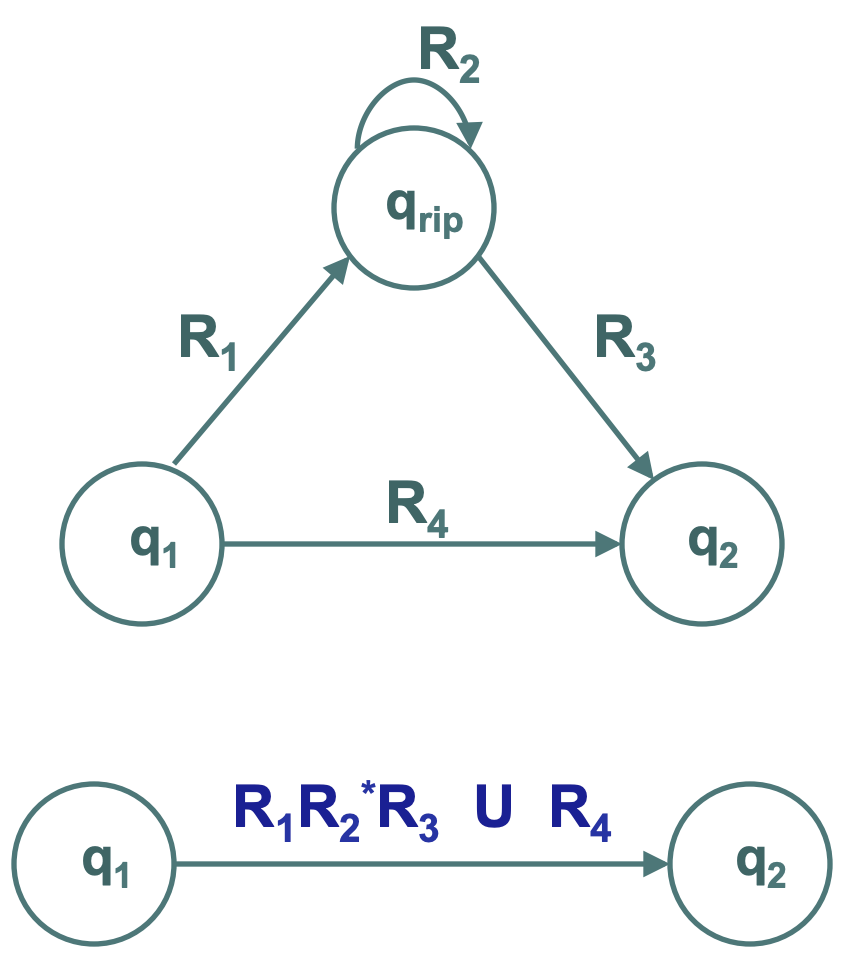
\includegraphics[scale=0.25]{rip.png}
    \end{minipage}
    \item Rip rip rip! Using the formula above.
\end{enumerate}

\subsubsection{RE to NFA}
Use process similar to induction.

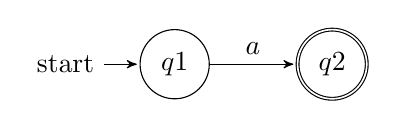
\begin{tikzpicture}[->,>=stealth',shorten >=1pt,auto,node distance=2cm,
        scale = 1,transform shape]

  \node[state,initial] (q1) {$q1$};
  \node[state,accepting] (q2) [right of=q1] {$q2$};
  \path (q1) edge              node {$a$} (q2);
\end{tikzpicture}

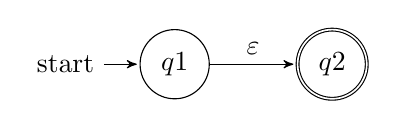
\begin{tikzpicture}[->,>=stealth',shorten >=1pt,auto,node distance=2cm,
        scale = 1,transform shape]
  \node[state,initial] (q1) {$q1$};
  \node[state,accepting] (q2) [right of=q1] {$q2$};

  \path (q1) edge              node {$\varepsilon$} (q2);
\end{tikzpicture}

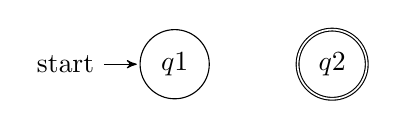
\begin{tikzpicture}[->,>=stealth',shorten >=1pt,auto,node distance=2cm,
        scale = 1,transform shape]

  \node[state,initial] (q1) {$q1$};
  \node[state,accepting] (q2) [right of=q1] {$q2$};
\end{tikzpicture}

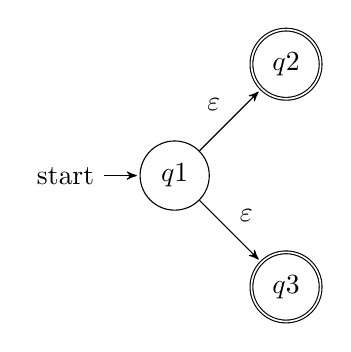
\begin{tikzpicture}[->,>=stealth',shorten >=1pt,auto,node distance=2cm,
        scale = 1,transform shape]
  \node[state,initial] (q1) {$q1$};
  \node[state,accepting] (q2) [above right of=q1] {$q2$};
  \node[state,accepting] (q3) [below right of=q1] {$q3$};

  \path (q1) edge              node {$\varepsilon$} (q2)
        (q1) edge              node {$\varepsilon$} (q3);
\end{tikzpicture}

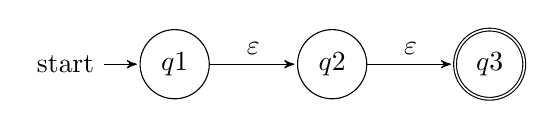
\begin{tikzpicture}[->,>=stealth',shorten >=1pt,auto,node distance=2cm,
        scale = 1,transform shape]
  \node[state,initial] (q1) {$q1$};
  \node[state] (q2) [right of=q1] {$q2$};
  \node[state,accepting] (q3) [right of=q2] {$q3$};

  \path (q1) edge              node {$\varepsilon$} (q2)
        (q2) edge              node {$\varepsilon$} (q3);
\end{tikzpicture}

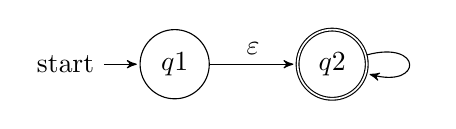
\begin{tikzpicture}[->,>=stealth',shorten >=1pt,auto,node distance=2cm,
        scale = 1,transform shape]
  \node[state,initial] (q1) {$q1$};
  \node[state,accepting] (q2) [right of=q1] {$q2$};

  \path (q1) edge              node {$\varepsilon$} (q2)
        (q2) edge[loop right]              node {} (q2);
\end{tikzpicture}

\subsection{Closure}
\subsubsection{Union using NFA}
\begin{itemize}
    \item $Q = Q_1 \cup Q_2 \cup \{q_{new}\}$
    \item $\Sigma = \Sigma_1 = \Sigma_2$
    \item $\delta(r,a)$ = 
    $\begin{cases}
    \delta_1(r,a) & \textrm{ if } r \in Q_1\\
    \delta_2(r,a) & \textrm{ if } r \in Q_2\\
    \{q_{01}, q_{02}\} & \textrm{ if } r = q_{new}, a = \varepsilon\\
    \emptyset & \textrm{ if } r=q_{new}, a \neq \varepsilon
    \end{cases}$
    \item $q_0 = q_{new}$
    \item $F = F_1 \cup F_2$
\end{itemize}

\subsection{Pumping Lemma}
\subsubsection{Formal}
If $A$ is a regular language, then there exists an integer $p$ where if $s$ from $A$ is any string of length at least $p$, then $s$ may be divided into three pieces, $s=xyz$, such that:
\begin{itemize}
    \item $\forall i \geq 0$, $xy^{i}z \in A$.
    \item $|y| > 0$
    \item $|xy| \leq p$
\end{itemize}
\subsubsection{Informal}
Given a regular language $A$, the pumping lemma holds. The pumping lemma says that if we have a long string (a string with length greater than the number of states), we know that there must be some loop in the machine, and we can partition the machine into three pieces, $xyz$, where y is the loop.
\begin{itemize}
    \item If we pump the loop 0 or more times, it is still in the language.
    \item The loop exists, in the sense that it has at least one state.
    \item The leadup to the loop and the loop combined fit into the machine.
\end{itemize}

\subsection{Proving nonregularity}
FSOC, assume that $A$ is regular. Then, the properties of pumping lemma apply, enumerate. Consider a long string $s=xyz$ (choose $s$) with an arbitrary partition up to $p$ that satisfies pumping lemma. If we pump it more or less (choose $i$), then it is no longer in the language.

\subsection{Other notes}
\begin{itemize}
    \item To show that reversed strings are closed under regular languages, we can just swap the arrows in a DFA, but cannot do so in NFA. This is because NFA has dead states.
\end{itemize}


\section{Context Free Languages}
\subsection{Properties}
\begin{itemize}
    \item Regular languages are a subset of context free languages.
    \item Consistency - generates all strings in language.
    \item Consistency - generates only strings in language.
    \item Ambiguous - string derived from grammar in fundamentally different ways. Show that either 1) give different parse trees or 2) different leftmost derivations.
\end{itemize}

\subsection{Context Free Grammar}
$G = (V, \Sigma, R, S)$
\begin{itemize}
    \item $V$ - variables, finite set of symbols, typically caps
    \item $\Sigma$ - terminals, finite set of symbols, disjoint from variables ($V \cap \Sigma = \emptyset$), typically lowercase
    \item $R$ - finite set of rules, e.g. $A \to B$
    \item $S \in V$ - start symbol
\end{itemize}
Start with $S$, derive by repeating rules until no more variables, only terminals.

\subsubsection{Parse Tree}
\begin{itemize}
    \item Leaves are terminals.
    \item Internal nodes are variables.
    \item Branches correspond to concatenation
\end{itemize}

\subsubsection{Chomsky Normal Form}
Equivalent to CFG. Basically, CFG with certain conditions. Conditions:
\begin{itemize}
    \item $A \to BC$
    \item $A \to a$
    \item $B,C$ cannot be $S$
    \item Only $S$ can go to $\varepsilon$
\end{itemize}

\subsection{Converting from RE to CFG}
\begin{itemize}
    \item $a = S \to a$
    \item $\varepsilon = S \to \varepsilon$
    \item $\emptyset = S \to S$
    \item $R_1 \cup R_2 = S \to S_1 | S_2$
    \item $R_1 \circ R_2 = S \to S_1 S_2$
    \item $R_1^* = S \to S_1 S$
\end{itemize}

\subsection{Push Down Automata}
$P = (Q, \Sigma, \Gamma, \delta, q_0, F)$
\begin{itemize}
    \item $Q$ = finite set of states
    \item $\Sigma$ = alphabet, finite set of symbols
    \item $\Gamma$ = stack alphabet, finite set of symbols
    \item $\delta: Q \times \Sigma_{\varepsilon} \times \Gamma_{\varepsilon} \to P(Q\times \Gamma_{\varepsilon})$ = transition function, e.g. $a, b\to c$
    \item $q_0$ = start state
    \item $F \subseteq Q$ = set of final states
\end{itemize}
\subsubsection{Useful transitions}
\begin{itemize}
    \item $\textrm{symbol } a, \textrm{ pop } b \to \textrm{push } c$ = take arrow if symbol in string is $a$ and top of stack is $b$. Pop $b$ off stack and push $c$.
    \item $a, \varepsilon \to \varepsilon$ = consume symbol, ignore stack
    \item $\varepsilon, \varepsilon \to b$ = consume no symbol, push onto stack
    \item $\varepsilon, b \to \varepsilon$ = consume no symbol, pop off of stack
    \item $\varepsilon, \varepsilon \to \varepsilon$ = consume no symbol, ignore stack
\end{itemize}

\subsection{Converting from CFG to PDA}
\begin{itemize}
    \item The general idea is that we place an empty marker on the stack and on top of that, the reverse of all possible generations. We put rules that consume the input $x, x\to \varepsilon$ to check if we can uncover the $\$$, meaning that it is a valid string.
    
    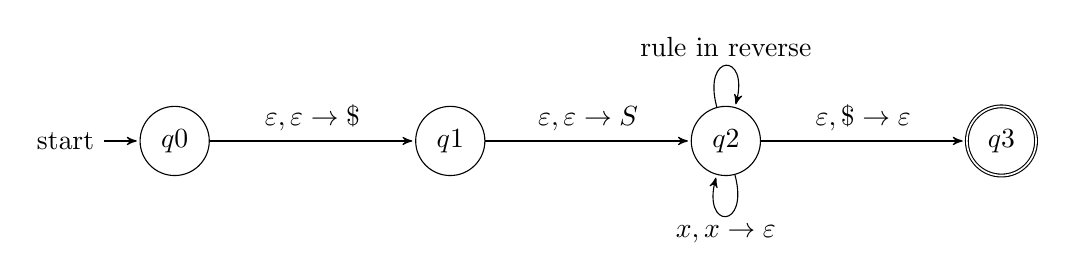
\begin{tikzpicture}[->,>=stealth',shorten >=1pt,auto,node distance=3.5cm,
        scale = 1,transform shape]

  \node[state,initial] (q0) {$q0$};
  \node[state] (q1) [right of=q0] {$q1$};
  \node[state] (q2) [right of=q1] {$q2$};
  \node[state,accepting] (q3) [right of=q2] {$q3$};

  \path (q0) edge              node {$\varepsilon, \varepsilon \to \$$} (q1)
        (q1) edge              node {$\varepsilon, \varepsilon \to S$} (q2)
        (q2) edge[loop above]              node {$\textrm{rule in reverse}$} (q2)
        (q2) edge              node {$\varepsilon, \$ \to \varepsilon$} (q3)
        (q2) edge[loop below]              node {$x, x \to \varepsilon$} (q2);

\end{tikzpicture}
\end{itemize}

\subsection{Converting from PDA to CFG}
A bit too involved, but know that it is possible.

\subsection{Other notes}
\begin{itemize}
    \item Stacks lack notion of emptiness, so often use \$ symbol emptiness\\
    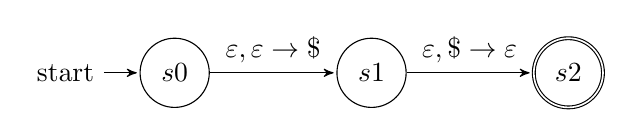
\begin{tikzpicture}[->,>=stealth',shorten >=1pt,auto,node distance=2.5cm,
        scale = 1,transform shape]

  \node[state,initial] (s0) {$s0$};
  \node[state] (s1) [right of=s0] {$s1$};
  \node[state,accepting] (s2) [right of=s1] {$s2$};

  \path (s0) edge              node {$\varepsilon, \varepsilon\to \$$} (s1)
        (s1) edge              node {$\varepsilon, \$ \to \varepsilon$} (s2);

\end{tikzpicture}
\end{itemize}


\end{document}
